\chapter{Device and Cloudlet Implementation}\label{chap:implementation}

This chapter describes a new version of the Gabriel software framework that we
developed for WCA applications.
Next, it examines DNNs that can be run on mobile devices, and how
these models can be used in WCA applications to reduce the bandwidth and
latency consumed by each WCA application user.

\section{Software Framework}

We developed a set of software libraries for WCA applications, called
Gabriel~\cite{gabriel_github}.
The primary feature of these libraries is to transmit data from mobile devices
to cloudlets.
WCA applications require responses shortly after a user completes a step, so
we always want to process the newest frame possible. We never want to build up
a queue of stale data to process. The library accomplishes this using a flow
control mechanism similar to the one proposed by \citet{ha2014}.

\subsection{Motivation}

The library we developed replaces an earlier implementation.
The code for this earlier implementation had become unmanageable.
It was tightly coupled around sending single image frames, and we
wanted the ability to send chunks of consecutive frames in order to support
activity recognition in WCA tasks.
We also needed multiple clients to share one cloudlet, which the old code did
not support.
Developing a new version of the platform allowed us to use modern technologies
such as Python 3, WebSockets, and asyncio.
A key goal with the new version of the platform was making it easy to work with.
We published server and client libraries to package repositories, so that
developers can easily include them in Python and Android code.
Our code includes a special case for Gabriel workflows that involve a single
cognitive engine, which allows this engine to be run with the server in the same
Python program.

\subsection{Implementation Details}

We use the abstractions of ``sources'' and ``cognitive engines.'' A source is
anything that produces data on a mobile device. It could be a stream from a
sensor such as a camera or microphone. A source might also be a filter that runs
on the device, analyzes all frames produced by a sensor, but then only forwards
some of these frames to the
cloudlet. We use the term ``early discard'' to refer to filters like
this. A cognitive engine runs on a cloudlet and processes data. A cognitive
engine will process one frame of data at a time. A frame could be a single
image, a short clip of audio and/or video, or set of readings from different
types of sensors.

All of the wearable cognitive assistance applications we have developed just
have a single cognitive engine processing images from a single camera source.
However, our framework supports workloads with multiple sources and multiple
cognitive engines. Multiple cognitive engines may consume data from the same
source, but we restrict each cognitive engine to consuming data from one source.
This reduces the complexity of cognitive engines.

Cognitive engines are all implemented in Python. Developers implement a single
function that takes a frame as its input parameter and returns a list of
results when it completes. Cognitive engines that do not need to return results
to mobile devices can just return an empty list.

\subsubsection{Flow Control}

Our flow control mechanism is
based on tokens. Clients have a set of tokens for every source. When a client
sends a frame to the cloudlet, it gives up a token for this source. The cloudlet
returns the relevant token when the function processing the frame returns.
A client will drop all frames from a source, until it gets a token for this
source. Clients and
cloudlets communicate using the The WebSocket Protocol~\cite{websocket}, which
is built on TCP.
Therefore, tokens will never be lost due to packet loss.

Applications that are very latency sensitive, such as
wearable cognitive assistance, will be run with a single token per source.
Applications that can tolerate higher latency can be run with more tokens.
Multiple tokens
will allow frames to be transmitted while the cloudlet is busy processing other
frames. This may cause frames to be buffered on the cloudlet, if the
cognitive engine takes a long time to process earlier frames. As a result, there
might be a significant amount of time between when a frame is captured and when
it gets processed. However, using multiple tokens does avoid periods where the
cloudlet does not have any frames to process because it is waiting for the next
frame to be sent over the network. Increasing
the number of tokens thus increases the possible delay before a frame gets
processed but reduces the amount of time the cloudlet has no frames to process,
when network latency is high.
The number of tokens is thus a parameter that will
increase the framerate for applications that can tolerate higher latency.

When multiple cognitive engines consume frames from the same source, the token
for a frame is returned when the first cognitive engine finishes processing the
frame.
A Client will only receive a result from the first cognitive engine that
finishes processing a frame, and it will not get additional results or tokens
when other engines finish processing the same frame. Our server library keeps a
queue of input frames for each source. When multiple clients produce frames from
the same source, such as two smartphones both capturing images with an RGB
camera, these frames are put into the same queue.
Figure~\ref{fig:queues} shows an example of how frames are inserted into queues.

\begin{figure}[h!]
  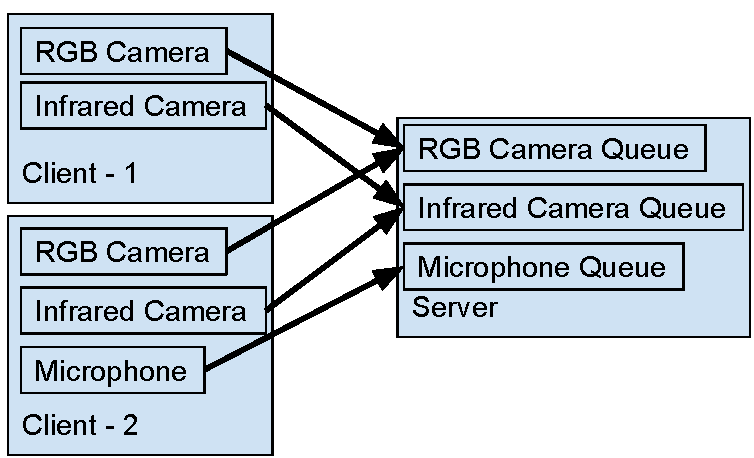
\includegraphics[width=8cm]{figures/queues.pdf}
  \caption{Two Gabriel clients that produce frames from multiple sensors.
    The arrows represent frames being inserted into queues on the server.
  }\label{fig:queues}
\end{figure}

A cognitive engine will process the
frame at the head of the queue for the source it consumes frames from. This
frame will be left at the head of the queue, so other cognitive engines that
consume frames from the same source will also process it. This frame is only
removed from the queue when a cognitive engine finishes processing it. The
engine that finishes processing the frame at the head of the queue will be the
first to get the next frame in the queue (if there is one).

This mechanism ensures that frames get consumed at the rate that the fastest
cognitive engine can process them.
If every cognitive engine took a frame from the queue without leaving it for
other engines, a slower engine would process frames that the fastest engine does
not.
This method also ensures that cognitive engines do not get stale
frames because they are slow. Cognitive engines always process the frame at the
head of the queue. If one engine is slow, and the queue gets advanced several
times while the slow engine is processing a single frame, the slow engine
ignores the frames it missed. Once this engine becomes free, it will start
processing the frame at the head of the queue at that time.

The fastest cognitive engine might process frames from the queue faster than
clients can deliver new ones.
This is especially likely when the number of clients is low, the network has
high latency and low bandwidth, and the number of tokens is set to a low value.
An easy solution to this problem is increasing the number of tokens.
However, this is not an option for applications that are latency sensitive, such
as WCA.
In this case, the fastest cognitive engine will have periods where it sits idle
while it waits to receive a new frame to process.

\subsubsection{Components}

Almost all of our applications use a single cognitive engine. Our server code
runs workflows like this as a single Python program. A WebSocket server is run
in the main process, and the cognitive engine is run in a separate process using
Python's multiprocessing module. Inter-process communication is done using the
multiprocessing module's Pipe function. For workloads that require multiple
cognitive engines (such as the one depicted in
Figure~\ref{fig:runtime_architecture}),
the WebSocket server is run as a standalone Python program and each cognitive
engine is run as a different Python program.
The Python programs communicate with each other using ZeroMQ~\cite{zmq}.
All Python programs can be run on a single cloudlet, or they can be run on
different cloudlets.

\begin{figure}[h!]
  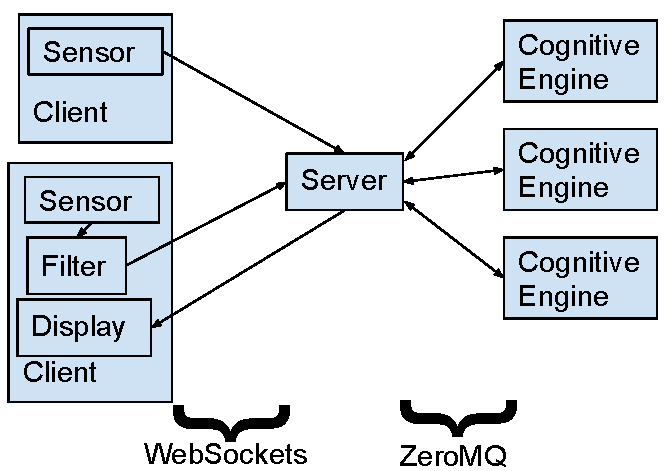
\includegraphics[width=8cm]{figures/runtime_architecture.pdf}
  \caption{A Gabriel workflow with two clients and three cognitive engines.
  }\label{fig:runtime_architecture}
\end{figure}

We have developed client libraries for Python and Android. These include
networking components that communicate with our server code using WebSockets.
The libraries also contain functions to capture images with a camera and
transmit the latest frame whenever a token is available. The Python library uses
OpenCV~\cite{opencv_library} to capture images while the Android library uses
CameraX~\cite{camerax}. Our Python code has been published to The Python Package
Index (PyPI)~\cite{gabriel_server, gabriel_python_client} and our Android code
has been published to Maven Central~\cite{gabriel_android_client}.

\section{Leveraging Mobile Device Hardware}

This section considers running shifting some (or all) of the computations for
WCA applications from cloudlets to mobile devices.
This leverages on-device computation to reduce bandwidth and cloudlet usage.

\subsection{Accuracy Comparisons}

We compare the accuracy of models and model pairs that developers can use in WCA
applications.
Some of these models can be run directly on mobile devices or on cloudlets,
while others can only be run on cloudlets.

\subsubsection{Running a Single Model}\label{sec:single_model}

In an attempt to develop extremely lightweight versions of our applications,
we considered using a single DNN, rather than the pipeline described in
\S\ref{sec:two_stage}.
We used data from four of our applications, which is summarized in
Table~\ref{tab:dataset_size}.
The training set contains images that were labeled with a bounding box around
the subassembly.
The test set contains images that are distinct from the training set, but were
not labeled with bounding boxes.
All images in the training and test sets were assigned a class label, indicating
the step of the task that was shown in the image.

\begin{table}
\begin{tabular}{|l||p{10.5cm}|l|l|}
  \hline
  & & \multicolumn{2}{c|}{Set Size}\\
  Name & Description & Training & Test \\
  \hline
  \hline
  Stirling & Assemble a heat engine from metal parts & 9598 & 10010\\
  Meccano & Build a model bike from metal parts & 15477 & 4490\\
  Toyplane & Build a model helicopter from 3D printed plastic parts & 55000 & 14996\\
  Sanitizer & Assemble a sanitizer for a smartphone from metal and plastic parts & 49956 & 60129\\
  \hline
\end{tabular}
  \caption{
    A summary of the data used for the experiments in this section.
    Set sizes are measured in number of images.
    Each dataset corresponds to one of our WCA applications.
  }\label{tab:dataset_size}
\end{table}

For each application, we trained a Resnet 50~\cite{He2016} image classifier,
three different sized EfficientDet~\cite{Tan2020} object detectors, a
Fast MPN-COV~\cite{Li_2018_CVPR} classifier, and a standalone Faster
R-CNN~\cite{frcnn} object detector.
We then evaluated these models on the test set for the relevant application.
When evaluating object detection results, we ignored bounding box coordinates
and just checked if the class label for the detected object with the highest
confidence score was correct.
Table~\ref{tab:standalone_accuracy} lists the accuracy of these models.

\begin{table}
\begin{tabular}{|l||l|l|l|l|}
\hline
  & Meccano & Stirling & Sanitizer & Toyplane\\
  \hline
  \hline
  Resnet 50 & 69.8\% & 26.3\% & 68.3\% & 56.4\%\\
  EfficintDet-Lite0 & \textbf{75.2\%} & 53.7\% & 79.3\% & 51.1\%\\
  EfficintDet-Lite1 & 71.1\% & \textbf{53.8\%} & 84.1\% & \textbf{63.5\%}\\
  EfficintDet-Lite2 & \textbf{75.2\%} & 49.6\% & \textbf{84.9\%} & 59.8\%\\
  \hline
\end{tabular}
  \caption{
    Classification accuracy for standalone DNN models.
    Accuracy is the percentage of images that the model classified correctly.
    The highest accuracy for each application is in bold.
  }\label{tab:standalone_accuracy}
\end{table}

\subsubsection{Running a Pipeline of Models}

The results in Table~\ref{tab:standalone_accuracy} leave a lot of room for
improvement.
We next evaluated an object detector and an image classifier used in a pipeline,
as described in \S\ref{sec:two_stage}.
Our standalone image classifiers were trained and tested
on uncropped images, while the image classifiers in our pipeline setup were
trained on images that were cropped to just contain the subassembly.
When testing the pipeline, we ran the object detector on uncropped images.
Then, we cropped the image around the bounding box returned by the object
detector, and then ran the image classifier on this cropped image.
Figure~\ref{fig:cropped_uncropped} shows examples of cropped and uncropped
images.
The results of these pipelines are presented in
Table~\ref{tab:pipeline_accuracy}.

\begin{figure}
  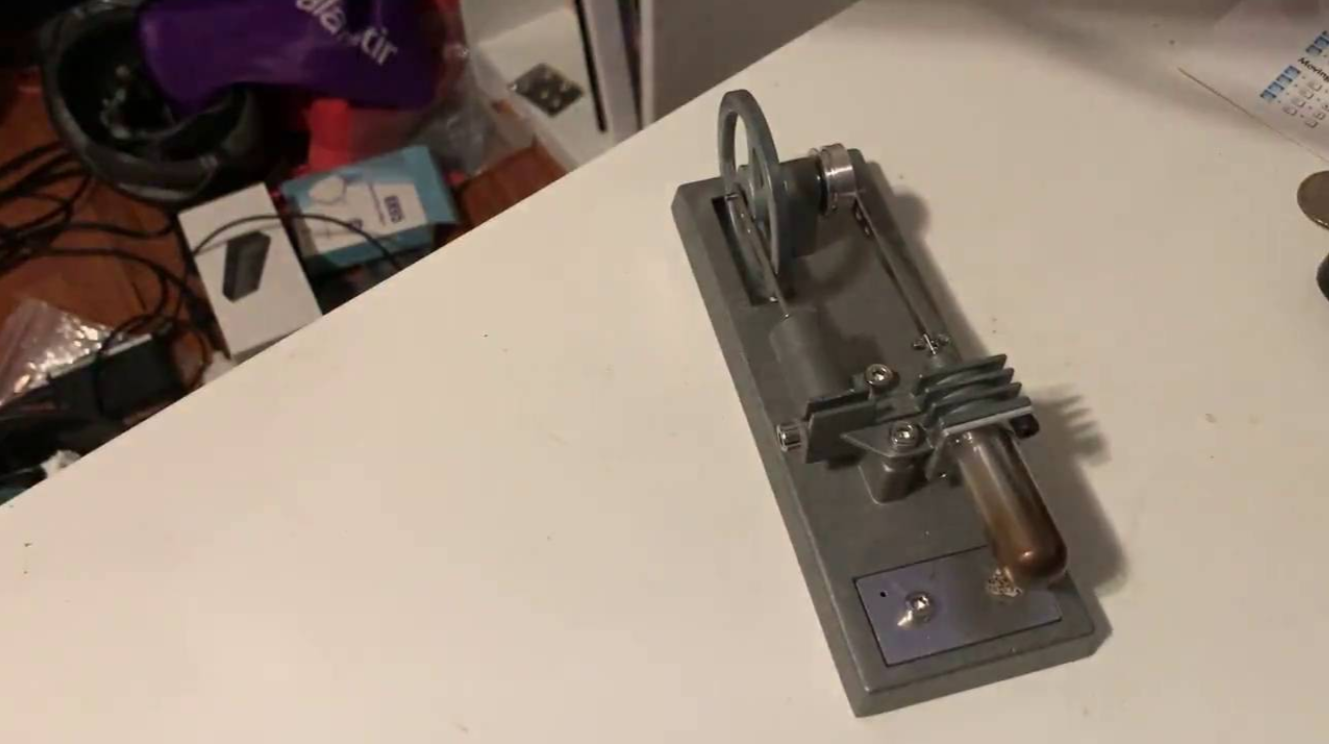
\includegraphics[width=7cm]{figures/stirling/uncropped.png}
  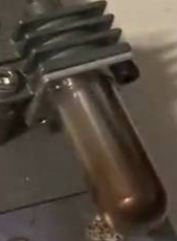
\includegraphics[width=3cm, left]{figures/stirling/cropped.png}
  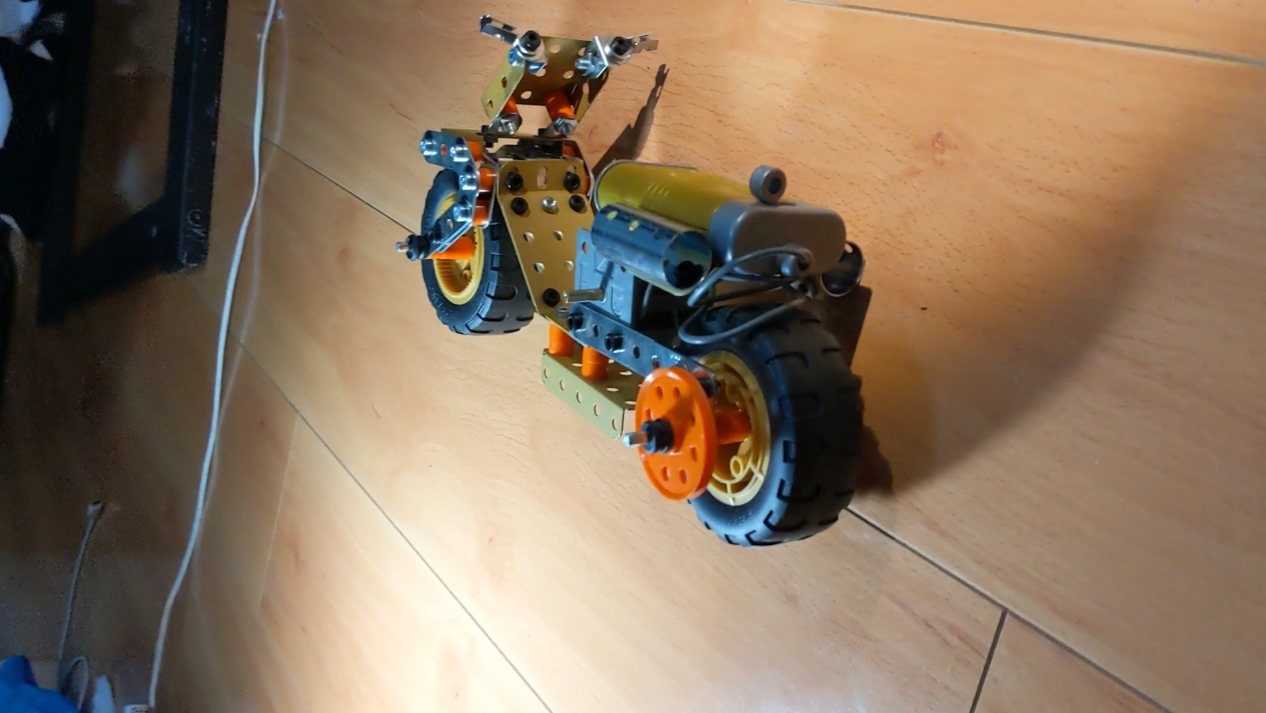
\includegraphics[width=7cm]{figures/erector/uncropped.png}
  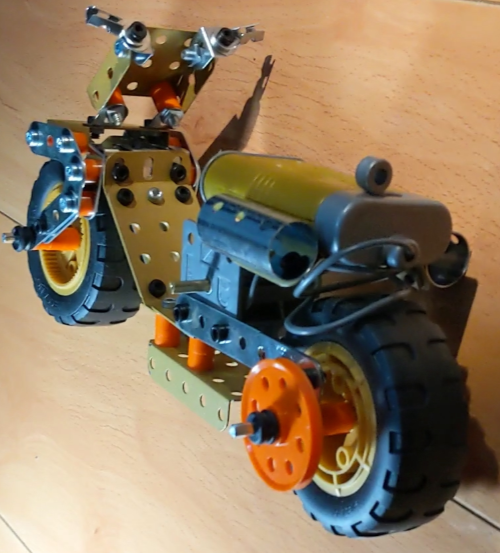
\includegraphics[width=3cm]{figures/erector/cropped.png}
  \caption{
    Uncropped (left) and Cropped (right) images showing steps from the Stirling
    and Meccano tasks.
  }\label{fig:cropped_uncropped}
\end{figure}

\begin{table}
\begin{tabular}{|l||l|l|l|l|}
  \hline
  & Meccano & Stirling & Sanitizer & Toyplane\\
  \hline
  \hline
  EfficientDet-Lite0 and Resnet 50 & 75.0\% & 85.1\% & 87.9\% & 69.8\%\\
  EfficientDet-Lite0 and Fast MPN-COV & 82.0\% & 78.4\% & 79.3\% & 77.2\%\\
  EfficientDet-Lite1 and Resnet 50 & 74.6\% & 70.3\% & 87.7\% & 70.9\%\\
  EfficientDet-Lite1 and Fast MPN-COV & 81.7\% & 66.6\% & 79.3\% & 77.7\%\\
  EfficientDet-Lite2 and Resnet 50 & 75.0\% & \textbf{91.0\%} & 89.1\% & 70.1\%\\
  EfficientDet-Lite2 and Fast MPN-COV & 81.5\% & 86.0\% & 80.6\% & 76.6\%\\
  Faster R-CNN and Fast MPN-COV & \textbf{84.5\%} & 80.9\% & \textbf{92.9\%} & \textbf{81.9\%}\\
  \hline
\end{tabular}
  \caption{
    Classification accuracy for pipelines consisting of an object detector,
    followed by an image classifier.
    Accuracy is the percentage of images that the model classified correctly.
    The highest accuracy for each application is in bold.
  }\label{tab:pipeline_accuracy}
\end{table}

The accuracy of the best pipeline was better than the accuracy of the best
standalone DNN for all of our applications.
Faster R-CNN and Fast MPN-COV was the best pipeline for all of our applications
except Stirling, where EfficientDet-Lite2 and Resnet 50 worked better.
This highlights the need for WCA application developers to determine the models
that work best for their specific application.

\subsection{On-device WCA}

The EfficientDet~\cite{Tan2020} object detector and Resnet 50~\cite{He2016}
image classifier can be run on certain Android devices using TensorFlow Lite.
This allows developers to create WCA applications that run some or all of their
computations on mobile devices instead of cloudlets.
However, Fast MPN-COV and Faster R-CNN cannot currently run on mobile
devices~\cite{tflite, torchscript}.

We developed versions of our applications that ran EfficientDet and Resnet 50
pipelines directly on mobile devices.
We profiled our applications on the three devices listed in
Table~\ref{tab:devices}.
All three devices run Android, which allowed us to re-use our code across all of
the devices.

\begin{table}
\begin{tabular}{|l||l|l|}
  \hline
  Device & Google Glass Enterprise Edition 2 & Magic Leap 2 \\
  \hline
  \hline
  Year Launched & 2019 & 2022 \\
  Weight & 51 g & 260 g \\
  Computing Hardware & Qualcomm Snapdragon XR1 & AMD Zen 2 and AMD RDNA 2 \\
  External Compute Pack & No & Yes \\
  Spatial Mapping & No & Yes \\
  \hline
\end{tabular}
\begin{tabular}{|l||l|}
  \hline
  Device & Vuzix Blade 2\\
  \hline
  \hline
  Year Launched & 2022\\
  Weight & 93 g \\
  Computing Hardware & Quad Core ARM CPU\\
  External Compute Pack & No\\
  Spatial Mapping & No\\
  \hline
\end{tabular}
  \caption{
    The smart glasses that we profiled our applications on. The values in the
    ``Computing Hardware'' row came from the tech specs advertised by the device
    manufacturer.
  }\label{tab:devices}
\end{table}

\subsubsection{Inference Time}\label{sec:mobile_inf_time}

We first measured the amount of time it took to process an image through the
two-DNN pipeline.
We accomplished this by storing our test set on the devices, and running code
that looped through each image.
Inside the loop, our code ran the pipeline of models that was being timed.
The code logged the elapsed time every 20 frames, based on Android's uptime
counter.
Each pipeline was run for five minutes.
Table~\ref{tab:mobile_inference} lists all of these times.

\begin{table}
\begin{tabular}{|l||l|l|l|}
  \hline
  & Google Glass EE 2 & Magic Leap 2 & Vuzix Blade 2\\
  \hline
  \hline
  EfficientDet-Lite0 and Resnet 50 & 480 $\pm$ 14 & 161 $\pm$ 3 & 2031 $\pm$ 27\\
  EfficientDet-Lite1 and Resnet 50 & 661 $\pm$ 46 & 183 $\pm$ 7 & 2423 $\pm$ 155\\
  EfficientDet-Lite2 and Resnet 50 & 958 $\pm$ 9 & 222 $\pm$ 3 & 3072 $\pm$ 73\\
  \hline
\end{tabular}
  \caption{
    Inference time for one frame, in milliseconds.
    For each cell, the average comes before the $\pm$ sign and the standard
    deviation comes after.
  }\label{tab:mobile_inference}
\end{table}

\citet{chen2017} conducted user studies to determine acceptable latency bounds
for WCA applications.
They found tight and loose latency bounds, which they describe as follows:
\begin{quotation}
``The tight bound represents an ideal target, below which the
user is insensitive to improvements, as measured, for example,
by impact on performance or ratings of satisfaction. Above
the loose bound, the user becomes aware of slowness, and
user experience and performance is significantly impacted.''
\end{quotation}
The tight latency bound for an assembly application was 600 ms, and the loose
bound was 2700 ms. Table~\ref{tab:mobile_accuracy} lists the largest pipeline
(in terms of DNN size)
that meets the these latency bounds on each device.

\begin{table}
\begin{tabular}{|l||l|l|l|}
  \hline
  & Tight Bound & Loose Bound\\
  \hline
  \hline
  Google Glass EE 2 & EfficientDet-Lite0 and Resnet 50 & EfficientDet-Lite2 and Resnet 50\\
  Magic Leap 2 & EfficientDet-Lite2 and Resnet 50 & EfficientDet-Lite2 and Resnet 50\\
  Vuzix Blade 2 & None & EfficientDet-Lite1 and Resnet 50\\
  \hline
\end{tabular}
  \caption{
    The largest pipeline that meets the tight and loose latency determined by
    \citet{chen2017}, for each of our devices.
    The accuracy of these pipelines is listed in
    Table~\ref{tab:pipeline_accuracy}.
  }\label{tab:mobile_accuracy}
\end{table}

\subsubsection{Power Consumption}\label{sec:mobile_power_consumption}

We measured the amount of power that each of these devices used while running
the pipelines in a loop.
As with our previous experiments, we ran each pipeline for five minutes.
None of these devices had user serviceable batteries, so we could not measure
power consumption based on the current and voltage that was being
supplied to the device by its charger.
Instead, we ran our code with the devices unplugged, and queried for current and
voltage readings from Android, using the BatteryManager class.
We multiplied the voltage and current to compute power.
Our code contained a background thread which logged the current and voltage
every 100 ms.
Figure~\ref{fig:power_graphs} shows graphs of power for all three devices,
sampled every 100 ms.
Each value repeats several times, which indicates that current and voltage
values were updated less frequently than 100 ms.
Unfortunately, this means that these measurements are somewhat crude.

\begin{figure}
  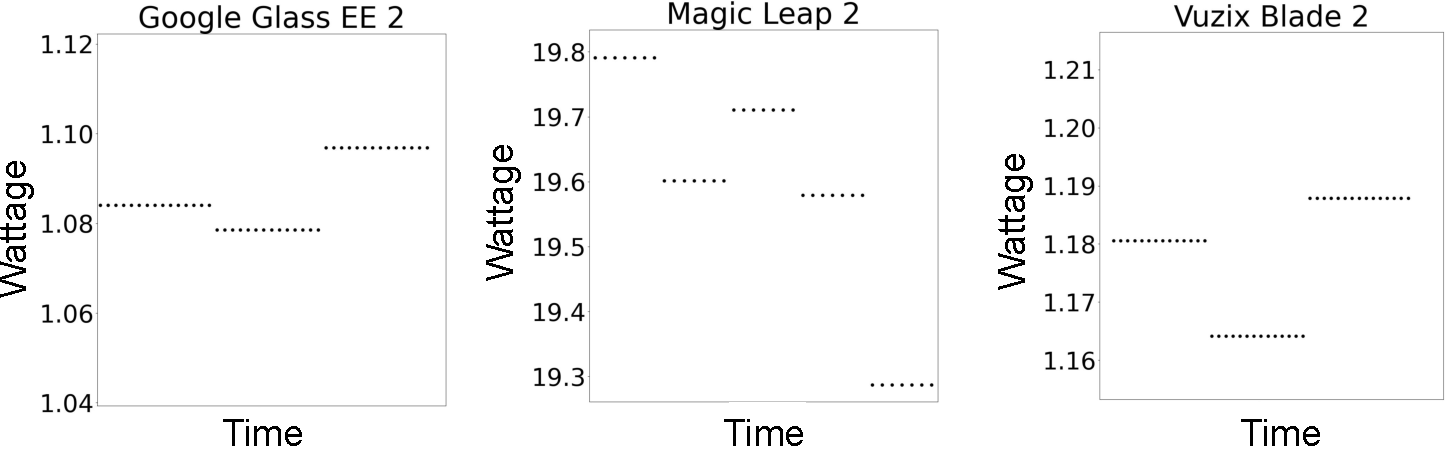
\includegraphics[width=\textwidth]{figures/power_graphs.pdf}
  \caption{Measured power values for our three headsets, running EfficientDet in
    a loop.
    Note that neither axes of these graphs start at zero.
    These values were sampled every 100 ms.
    The repeated values indicate that the current and voltage readings that
    Android provides access to are updated less frequently than 100 ms.
    As we describe in Section~\ref{sec:mobile_power_consumption}, the Magic Leap
    consumed significantly more power than the other devices that we tested.
  }\label{fig:power_graphs}
\end{figure}

Table~\ref{tab:mobile_power} lists the power values for each pipeline, running
on all three devices.
The baseline measurements were recorded for an application that showed an empty
Android activity, but did not do anything aside from recording current and
voltage values in a background thread.
Table~\ref{tab:mobile_power_pi} lists the percentage increase in power
consumption above the baseline, for running each pipeline.
Percentage increase was calculated using the formula:
\[
  \frac{\text{Pipeline Wattage} - \text{Baseline Wattage}}{
    \text{Baseline Wattage}}
\]

\begin{table}
\begin{tabular}{|l||l|l|l|}
  \hline
  & Google Glass EE 2 & Magic Leap 2 & Vuzix Blade 2\\
  \hline
  \hline
  Baseline & 0.61 $\pm$ 0.13 & 15.1 $\pm$ 0.46 & 0.84 $\pm$ 0.15\\
  EfficientDet-Lite0 and Resnet 50 & 1.43 $\pm$ 0.35 & 18.54 $\pm$ 0.37 & 1.18 $\pm$ 0.10\\
  EfficientDet-Lite1 and Resnet 50 & 1.26 $\pm$ 0.29 & 18.41 $\pm$ 0.22 & 1.24 $\pm$ 0.16\\
  EfficientDet-Lite2 and Resnet 50 & 1.26 $\pm$ 0.27 & 18.55 $\pm$ 0.16 & 1.22 $\pm$ 0.13\\
  \hline
\end{tabular}
  \caption{
    Average power consumption, in Watts.
    For each cell, the average comes before the $\pm$ sign and the standard
    deviation comes after.
    These measurements were recorded while the mobile device was running the
    full pipeline.
    The baseline application did not carry out any computation.
  }\label{tab:mobile_power}
\end{table}

\begin{table}
\begin{tabular}{|l||l|l|l|}
  \hline
  & Google Glass EE 2 & Magic Leap 2 & Vuzix Blade 2\\
  \hline
  \hline
  EfficientDet-Lite0 and Resnet 50 & 134\% & 23\% & 41\%\\
  EfficientDet-Lite1 and Resnet 50 & 106\% & 22\% & 48\%\\
  EfficientDet-Lite2 and Resnet 50 & 107\% & 23\% & 45\%\\
  \hline
\end{tabular}
  \caption{
    The percentage increase of power consumption, above the baseline.
  }\label{tab:mobile_power_pi}
\end{table}

The Magic Leap 2 consumed over 15 watts running the baseline application.
The device's depth sensors might have consumed some of this power, or it could
have been spatial mapping code running in the background.
None of the pipelines increased the Magic Leap 2's power usage by more than 25\%
of the power consumed by the baseline.
The most dramatic increase over baseline power usage was for EfficientDet-Lite0
and Resnet 50 on Google Glass EE 2, with an average power usage of 1.43 Watts.
However, this is still a reasonable amount of power.
A 3.2 Wh battery can supply 1.43 Watts for over two hours.

WCA application developers should not be dissuaded from running DNNs on mobile
devices, due to power consumption.

\subsection{Split Computing}

Split Computing offers a middle ground between offloading all computations to a
server, and carrying out all computations locally.
Instead, split computing uses a lightweight ``head,'' that runs lightweight
computations on the mobile device, and a heavyweight ``tail,'' that runs the
remainder of the computations on a more powerful server.

A large body of work exists exploring split computing applications.
Odyssey~\cite{Noble1997} modified the Janus speech recognition application to
operate in one of three modes.
In one of the modes, a preliminary phase of speech
processing was done locally (i.e., the head), and the extracted
information was shipped to a remote server for the completion of the
recognition process (i.e., the tail).
For certain combinations of
network bandwidth and device/server capabilities, this split offered
lower end-to-end latency than fully local or fully remote execution.
Several subsequent efforts in split computing~\cite{Balan2002, Flinn2001,
  Flinn2003b, Narayanan2003, Goyal2004, Su2005, Ok2007, Balan2007,
  Kristensen2008} were surveyed in 2012~\cite{Flinn2012}.

More recently, machine learning researchers have examined how DNN models can be
split across mobile devices and servers~\cite{Kang2017, Hsu2019, Eshratifar2019,
  Matsubara2019}.
These works partition the DNNs such that the output from the subset of the
network that runs on the mobile device (the head) is smaller than the
original input to the network.
We will henceforth refer to the output from the head as an embedding.
Transmitting the embedding to the server, instead of the original input saves
bandwidth.
The embedding is a compressed representation of the input, that the remainder of
the network (the tail) can process accurately.
However, there is no clear way to convert an embedding back to the original
input.
A 2022 survey~\cite{Matsubara2022} discusses a number of recent works on split
computing for DNNs.
Unfortunately, modifying the architecture of a DNN for split computing is
difficult~\cite{Matsubara2020}.
Split architectures exist for common computer vision tasks like object detection
and image classification.
However, many developers lack the skills to create split architectures for tasks
that such architectures don't already exist for.

Implementing the pipeline described in \S\ref{sec:two_stage} using a split
object detector is impractical.
The output from a split object detector just contains the bounding box
coordinates and class labels for detected objects.
There is no way for the server to obtain a cropped image from the original
embedding that was sent to the cloudlet.
Our application would either have to send the entire image to the cloudlet along
with the embedding, or it would have to send the bounding box coordinates back
to the mobile device, and have the mobile device send the cropped image in some
form to run the classifier.
The former approach eliminates all of the bandwidth savings that split computing
offers; while the latter approach requires a second round trip to the mobile
device, which increases latency.

We instead realized split computing by running an EfficientDet object detector
on a mobile device, and a Fast MPN-COV classifier on a cloudlet.
The client that runs on the mobile device crops images around the bounding box
with the highest confidence score, so only the detected subassembly remains in
the image.
This cropped image is then sent to the cloudlet, instead of the uncropped
original.
If the object detector does not find a subassembly in the image, the client does
not send anything to the cloudlet.

\subsubsection{Bandwidth Savings}

We compared the bandwidth required to transmit all images in full and the
bandwidth required to transmit the cropped images from our split computing
strategy.
For each of the four applications, we ran the EfficidntDet-Lite0 object detector
that was trained for this application on the full test set.
We recorded the number of bytes required to transmit the images cropped around
the subassemblies detected by the model, and compared this with the number of
bytes required to transmit the entire test set.
Table~\ref{tab:bandwidth} lists the bandwidth savings percentages, which were
calculated using the formula:
\[
  \frac{\text{Bytes for full images} - \text{Bytes for cropped images}}{
    \text{Bytes for full images}}
\]

\begin{table}
  \begin{tabular}{|l|l|l|l|}
  \hline
  Stirling & Meccano & Toyplane & Sanitizer\\
  \hline
  \hline
  79.2\% & 52.3\% & 86.8\% & 94.2\%\\
  \hline
\end{tabular}
\caption{
  The bandwidth saved by images cropped around the bounding boxes returned by
  EfficientDet-Lite0.
}\label{tab:bandwidth}
\end{table}

The bandwidth savings achieved by this strategy is content-dependant.
The distance between the camera and the object being assembled will change how
large a subassembly appears in the image, and this will directly impact the
number of bytes required to transmit the cropped image.
The bandwidth savings of techniques such as image compression or DNN-based split
computing vary less based on the specific content in an image.

Transmitting cropped images required less than 50\% of the bandwidth than
the uncropped images would have required, for all of our datasets.
The savings was over 90\% for the Sanitizer dataset.
In many cases, this significant bandwidth savings will be worth the reduction in
accuracy (presented in Table~\ref{tab:thin_accuracy}).

\subsubsection{Inference Time}

We measured the inference time of our split computing pipelines with code that
ran the pipelines in a loop, similar to our measurements in
Section~\ref{sec:mobile_inf_time}.
The loop runs through the images in our test set, and processes each one locally
with an object detector.
After an image is processed by the object detector, it is cropped if the
detector finds a subassembly with high confidence.
The crop is then sent to the cloudlet, where it is processed by the classifier.
After sending a cropped image to the cloudlet, the mobile device immediately
starts processing the next image.
However, we used a single token for Gabriel's flow control.
The mobile client cannot send a new cropped image to the cloudlet before the
cloudlet finishes processing the previous cropped image.
In cases where the client is ready with the next cropped image before the
cloudlet has finished processing the last one that was sent, the client will
wait for the cloudlet to finish processing the last image before the client
sends the next one.

The mobile devices were connected to the internet over Wi-Fi while the cloudlet
had a wired connection to the internet.
The ping time between the mobile device and the cloudlet was under 0.5 ms.
The cloudlet had an an Intel Intel Xeon E5–2699 CPU and a GeForce GTX 1080 Ti
GPU.

As with our other measurements, we ran each pipeline and device combination for
five minutes.
We logged the elapsed time every 20 iterations of the loop, and then divided the
elapsed time by 20 to compute the per-frame inference time.
Table~\ref{tab:split_time} lists the averages and standard deviations of the
per-frame inference times.
Table~\ref{tab:split_latency_bound} lists the most computationally intensive
split pipeline that meets the latency bounds from \citet{chen2017} on each
device.

\begin{table}
\begin{tabular}{|l||l|l|l|}
  \hline
  & Google Glass EE 2 & Magic Leap 2 & Vuzix Blade 2\\
  \hline
  \hline
  EfficientDet-Lite0 and Fast MPN-COV & 308 $\pm$ 22 & 106 $\pm$ 7 & 1120 $\pm$ 47\\
  EfficientDet-Lite1 and Fast MPN-COV & 622 $\pm$ 186 & 133 $\pm$ 6 & 1778 $\pm$ 210\\
  EfficientDet-Lite2 and Fast MPN-COV & 779 $\pm$ 38 & 154 $\pm$ 4 & 2156 $\pm$ 65\\
  \hline
\end{tabular}
  \caption{
    Inference time for one frame, in milliseconds.
    The EfficientDet models were run on the device, then crops were sent to the
    cloudlet, where they were processed by Fast MPN-COV.
    These values include the DNN processing times on the device and cloudlet, as
    well as the time to send cropped images to the cloudlet and send results
    back to the mobile device.
    For each cell, the average comes before the $\pm$ sign and the standard
    deviation comes after.
  }\label{tab:split_time}
\end{table}

\begin{table}
\begin{tabular}{|l||l|l|l|}
  \hline
  & Tight Bound & Loose Bound\\
  \hline
  \hline
  Google Glass EE 2 & EfficientDet-Lite0 and Fast MPN-COV & EfficientDet-Lite2 and Resnet 50\\
  Magic Leap 2 & EfficientDet-Lite2 and Resnet 50 & EfficientDet-Lite2 and Resnet 50\\
  Vuzix Blade 2 & None & EfficientDet-Lite2 and Resnet 50\\
  \hline
\end{tabular}
  \caption{
    The most computationally intensive split pipeline that meets the tight and
    loose latency determined by \citet{chen2017}, for each of our devices.
    The accuracy of these pipelines is listed in
    Table~\ref{tab:pipeline_accuracy}.
  }\label{tab:split_latency_bound}
\end{table}

\subsubsection{Power Consumption}

Similar to Section~\ref{sec:mobile_power_consumption}, we measured power
consumption using a background thread that obtained current and voltage values
from Android every 100 ms.
Our power measurements were just made on the mobile devices, and the power
consumed by the cloudlet was not measured.
Table~\ref{tab:mobile_power} lists the averages and standard deviations of our
power measurements, while Table~\ref{tab:mobile_power_percentage} lists the
percentage increase over the baseline.

\begin{table}
\begin{tabular}{|l||l|l|l|}
  \hline
  & Google Glass EE 2 & Magic Leap 2 & Vuzix Blade 2\\
  \hline
  \hline
  Baseline & 0.61 $\pm$ 0.13 & 15.1 $\pm$ 0.46 & 0.84 $\pm$ 0.15\\
  EfficientDet-Lite0 and Fast MPN-COV & 1.37 $\pm$ 0.11 & 18.03 $\pm$ 0.32 & 1.27 $\pm$ 0.10\\
  EfficientDet-Lite1 and Fast MPN-COV & 1.23 $\pm$ 0.15 & 18.31 $\pm$ 0.21 & 1.22 $\pm$ 0.10\\
  EfficientDet-Lite2 and Fast MPN-COV & 1.21 $\pm$ 0.16 & 18.76 $\pm$ 0.25 & 1.24 $\pm$ 0.12\\
  \hline
\end{tabular}
  \caption{
    Average power consumption, in Watts.
    For each cell, the average comes before the $\pm$ sign and the standard
    deviation comes after.
    These measurements were recorded while the mobile device ran the object
    detector and then sent cropped images to the cloudlet, which then ran the
    image classifier.
    The baseline application did not carry out any computation.
  }\label{tab:mobile_power}
\end{table}

\begin{table}
\begin{tabular}{|l||l|l|l|}
  \hline
  & Google Glass EE 2 & Magic Leap 2 & Vuzix Blade 2\\
  \hline
  \hline
  EfficientDet-Lite0 and Fast MPN-COV & 125\% & 19\% & 51\%\\
  EfficientDet-Lite1 and Fast MPN-COV & 102\% & 21\% & 45\%\\
  EfficientDet-Lite2 and Fast MPN-COV & 98\% & 24\% & 48\%\\
  \hline
\end{tabular}
  \caption{
    The percentage increase of power consumption, above the baseline.
  }\label{tab:mobile_power_percentage}
\end{table}

These values are similar to the power values for the pipelines that ran entirely
on mobile devices.
Split computing does not offer a significant reduction in power consumption
compared to running DNNs entirely on mobile devices.
Our discussion about power values from
Section~\ref{sec:mobile_power_consumption} applies to these values as well.

\subsection{Thin Clients}

This section compares our device-only implementations of WCA applications with
split computing implementations, and a thin client that runs both DNNs on a
cloudlet.

\subsubsection{Accuracy}

Table~\ref{tab:thin_accuracy} lists the accuracies for the thin client and the
highest accuracies for device-only and split computing pipelines.
The thin client achieved the best performance for all applications except for
Stirling.
The best performing pipeline for Stirling can be run in all three
configurations.

\begin{table}
\begin{tabular}{|l||l|l|l|l|}
  \hline
  & Meccano & Stirling & Sanitizer & Toyplane\\
  \hline
  \hline
  Best device-only pipeline & 75.0\% & 91.0\% & 89.1\% & 70.1\%\\
  Best split computing pipeline & 82.0\% & 91.0\% & 89.1\% & 77.7\%\\
  Thin client & 84.5\% & 91.0\% & 92.9\% & 81.9\%\\
  \hline
\end{tabular}
  \caption{
    Classification accuracy for pipelines consisting of an object detector,
    followed by an image classifier.
    Accuracy is the percentage of images that the model classified correctly.
  }\label{tab:thin_accuracy}
\end{table}

\subsubsection{Inference Time}

Table~\ref{tab:thin_times} lists the inference times for all three devices running
the thin client for five minutes.
These times include transmitting images to the cloudlet, processing them there,
and then transmitting results back to the mobile device.
As with our other time measurements, the applications were run for five minutes,
and elapsed time was recorded every 20 frames.
These values were well below the tight latency bounds on all three devices.

\begin{table}
\begin{tabular}{|l||l|l|l|}
  \hline
  Google Glass EE 2 & Magic Leap 2 & Vuzix Blade 2\\
  \hline
  \hline
  166 $\pm$ 8 & 150 $\pm$ 8 & 203 $\pm$ 9\\
  \hline
\end{tabular}
  \caption{
    Inference time for one frame, in milliseconds, for the thin client.
    For each cell, the average comes before the $\pm$ sign and the standard
    deviation comes after.
  }\label{tab:thin_times}
\end{table}

The Vuzix Blade 2 could not meet the tight latency bound when running any of the
split computing or device-only pipelines that we tested.
The thin client was the only way we were able to meet the tight latency bound
with the Vuzix Blade 2.
However, the Google Glass EE 2 and Magic Leap 2 were able to meet the tight
latency bound with some of the split computing and device-only pipelines that we
tested.

\subsubsection{Power Consumption}

Power measurements for the thin client, averaged over five minute runs, are
listed in Table~\ref{tab:thin_power}.
Running the thin client on the Vuzix Blade 2 consumed more power than running
the baseline application, but less power than running any of the device-only or
split computing pipelines.
The Google Glass EE 2 consumed a similar amount of power running the thin client
as it did when running the device-only and split computing pipelines.
The thin client on the Magic Leap 2 consumed slightly less power than the
baseline application.
There isn't a clear explanation for why this would have happened, but the
difference is fairly small.

\begin{table}
\begin{tabular}{|l||l|l|l|}
  \hline
  & Google Glass EE 2 & Magic Leap 2 & Vuzix Blade 2\\
  \hline
  \hline
  Baseline & 0.61 $\pm$ 0.13 & 15.1 $\pm$ 0.46 & 0.84 $\pm$ 0.15\\
  Thin Client & 1.30 $\pm$ 0.41 & 14.26 $\pm$ 0.33 & 1.17 $\pm$ 0.09\\
  \hline
\end{tabular}
  \caption{
    Average power consumption, in Watts.
    For each cell, the average comes before the $\pm$ sign and the standard
    deviation comes after.
    These measurements were recorded while the mobile device sent an image to
    the cloudlet, the cloudlet ran the two DNNs, and then sent the result back
    to the mobile device.
    The baseline application did not carry out any computation.
  }\label{tab:thin_power}
\end{table}

\section{Summary}

Our new implementation of Gabriel is designed to be maintainable and easy to
use.
In addition, it allows connections from multiple users at the same time, which
was previously unsupported.

Certain DNNs can run on mobile devices.
This enables WCA applications to run entirely on a mobile device.
Another option is to split the computation across a mobile device and a
cloudlet.
These options reduce the amount of network bandwidth that the application
consumes.
We found DNNs that can run on certain mobile devices with acceptable latency.
However, these models were often less accurate than the DNNs that require more
powerful servers.

We achieved the best performance for three out of our four applications
offloading all computations to a cloudlet.
However, cloudlet resources and bandwidth are limited resources.
Split computing offers a significant bandwidth savings, with a modest cost in
accuracy.
It is also possible to run WCA applications entirely on a mobile device, but
this hurts accuracy significantly.
